% ============================================================
% 22-de-casteljau-makie-explained.tex
% Compile with:  pdflatex -shell-escape 22-de-casteljau-makie-explained.tex
% The PNG must be in the same folder. Run twice for TOC.
% ============================================================

\documentclass[12pt, a4paper]{article}

\usepackage[T1]{fontenc}
\usepackage[utf8]{inputenc}
\usepackage{lmodern}
\usepackage[top=2.5cm, bottom=2.5cm, left=2.8cm, right=2.8cm]{geometry}
\usepackage{graphicx}
\usepackage{float}
\usepackage[dvipsnames]{xcolor}

\definecolor{codebg}{RGB}{248,248,248}
\definecolor{rulecolor}{RGB}{180,180,180}
\definecolor{examplebg}{RGB}{240,248,255}
\definecolor{examplerule}{RGB}{100,149,237}
\definecolor{notebg}{RGB}{255,250,230}
\definecolor{noterule}{RGB}{210,180,50}

\usepackage{minted}
\setminted[julia]{
  bgcolor=codebg, frame=leftline, framerule=1.5pt,
  rulecolor=rulecolor, linenos=false, fontsize=\small,
  breaklines=true, tabsize=4, style=friendly,
}

\usepackage{amsmath}
\usepackage{amssymb}
\usepackage{tikz}
\usetikzlibrary{shapes.geometric, arrows.meta, positioning}
\usepackage{mdframed}

\newmdenv[backgroundcolor=examplebg, linecolor=examplerule,
  linewidth=1.5pt, leftline=true, rightline=false,
  topline=false, bottomline=false,
  innerleftmargin=10pt, innerrightmargin=8pt,
  innertopmargin=6pt, innerbottommargin=6pt,
  skipabove=6pt, skipbelow=4pt]{examplebox}

\newmdenv[backgroundcolor=notebg, linecolor=noterule,
  linewidth=1.5pt, leftline=true, rightline=false,
  topline=false, bottomline=false,
  innerleftmargin=10pt, innerrightmargin=8pt,
  innertopmargin=6pt, innerbottommargin=6pt,
  skipabove=6pt, skipbelow=4pt]{notebox}

\usepackage[colorlinks=true, linkcolor=black, urlcolor=MidnightBlue]{hyperref}
\usepackage{booktabs}
\usepackage{needspace}
\usepackage{parskip}
\usepackage{titlesec}
\usepackage{fancyhdr}
\usepackage{datetime2}

\titleformat{\section}
  {\large\bfseries\color{MidnightBlue}}{\thesection.}{0.6em}{}
  [\vspace{-4pt}\rule{\linewidth}{0.4pt}]
\titleformat{\subsection}
  {\normalsize\bfseries\color{BrickRed}}{\thesubsection.}{0.5em}{}
\titleformat{\subsubsection}
  {\normalsize\bfseries}{\thesubsubsection.}{0.5em}{}

\pagestyle{fancy}
\fancyhf{}
\rhead{\textcolor{gray}{\small 22-de-casteljau-makie-explained}}
\lhead{\textcolor{gray}{\small De Casteljau Quartic 3-D --- CairoMakie}}
\cfoot{\thepage}
\renewcommand{\headrulewidth}{0.3pt}

\newcommand{\cd}[1]{\texttt{#1}}

\title{%
  \vspace{1cm}
  {\LARGE\bfseries De Casteljau Algorithm: Quartic (3-D)}\\[0.4em]
  {\large CairoMakie Visualisation}\\[0.4em]
  {\large Code and Plot Explanation for Julia Beginners}\\[0.4em]
  {\normalsize\texttt{22-de-casteljau-makie.jl}}
}
\author{E.R.\ Nurwijayadi}
\date{\DTMtoday}

\begin{document}

\maketitle
\thispagestyle{empty}

\begin{center}
\textit{Directed and curated by E.R.\ Nurwijayadi.
Code and explanations AI-generated.}
\end{center}

\begin{center}
\begin{minipage}{0.85\textwidth}
\small
This document explains \cd{22-de-casteljau-makie.jl}.
This is the most complex script in the series so far:
the De Casteljau algorithm applied to a \emph{quartic}
(degree-4) curve in 3-D space.
A quartic requires \textbf{four} reduction levels instead
of two.
New concepts: the general \cd{reduce\_level} function,
\cd{getfield} for dynamic named-tuple access, colour-with-alpha
tuples, and NaN dummy lines for legend entries.
\end{minipage}
\end{center}

\vspace{1em}\hrule\vspace{1.5em}
\tableofcontents
\newpage


% =============================================================
\needspace{8\baselineskip}
\section{The Plot}
% =============================================================

\begin{figure}[H]
  \centering
  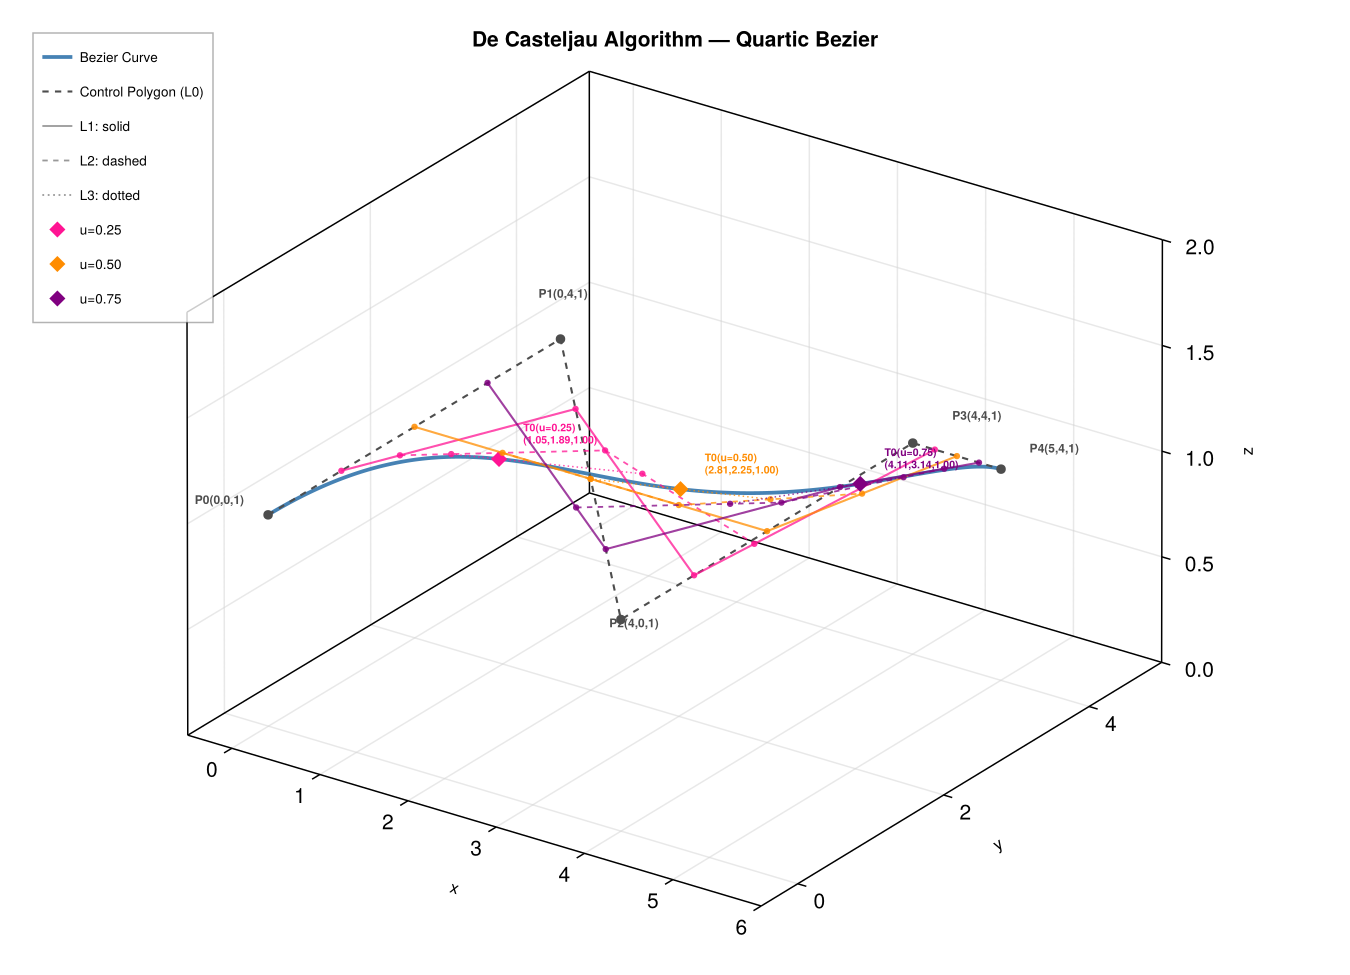
\includegraphics[width=0.95\linewidth]{22-bezier-decasteljau-quartic-makie.png}
  \caption{De Casteljau algorithm on a quartic B\'ezier in 3-D.
           Three snapshots at $u=0.25$ (pink), $u=0.50$ (orange),
           $u=0.75$ (purple). Each snapshot shows levels L1
           (solid), L2 (dashed), L3 (dotted), and the final
           curve point T0 (diamond).}
  \label{fig:dc-quartic}
\end{figure}


% =============================================================
\needspace{8\baselineskip}
\section{The De Casteljau Algorithm on a Quartic Curve}
% =============================================================

\textit{Script~12 showed De Casteljau on a quadratic curve ---
two control points became one in two steps.
A quartic curve has five control points, so the algorithm
needs four reduction steps.}

For a quartic B\'ezier with control points
$P_0, P_1, P_2, P_3, P_4$, the De Casteljau algorithm
at parameter $u$ proceeds as follows:

\textbf{Level 0 (L0):} 5 points --- the original control polygon.

\textbf{Level 1 (L1):} 4 points --- interpolate adjacent pairs from L0:
\[
  Q^1_i = (1-u)\,P_i + u\,P_{i+1} \quad i = 0,1,2,3
\]

\textbf{Level 2 (L2):} 3 points --- interpolate adjacent pairs from L1:
\[
  Q^2_i = (1-u)\,Q^1_i + u\,Q^1_{i+1} \quad i = 0,1,2
\]

\textbf{Level 3 (L3):} 2 points --- interpolate adjacent pairs from L2:
\[
  Q^3_i = (1-u)\,Q^2_i + u\,Q^2_{i+1} \quad i = 0,1
\]

\textbf{Level 4 (L4):} 1 point --- the final curve point:
\[
  T_0 = (1-u)\,Q^3_0 + u\,Q^3_1
\]

Each level is one row shorter than the previous.
The pattern ``$n$ points $\to$ $n-1$ points'' is exactly
what \cd{reduce\_level} implements.

\begin{notebox}
\textbf{Generalisation.}
This same pattern works for any degree $n$: apply
\cd{reduce\_level} exactly $n$ times.
The code is identical for quadratic, cubic, quartic,
or any higher degree --- only the number of calls changes.
\end{notebox}


% =============================================================
\needspace{8\baselineskip}
\section{Reading the Plot}
% =============================================================

\needspace{5\baselineskip}
\subsection{The layers}

\textbf{Blue curve} --- the quartic B\'ezier, 300 sample points.

\textbf{Gray dashed polygon} --- L0, the original 5 control points
connected by dashed lines. Labelled P0--P4.

\textbf{Coloured solid lines (L1)} --- for each snapshot colour,
the 4 L1 interpolation segments.

\textbf{Coloured dashed lines (L2)} --- the 3 L2 segments.

\textbf{Coloured dotted lines (L3)} --- the 2 L3 segments.

\textbf{Coloured diamonds (T0)} --- the final L4 point ---
the curve point at that $u$ value, sitting exactly on
the blue curve.

The legend has two kinds of entries:
line style entries (L1 solid, L2 dashed, L3 dotted)
shown in grey, and point entries (the three diamonds)
shown in their snapshot colours.

\needspace{5\baselineskip}
\subsection{Worked example: $u = 0.50$ (orange)}

At $u = 0.5$ all interpolations are midpoints.

\begin{examplebox}
\textbf{L1} (midpoints of L0 edges):
\begin{align*}
  Q^1_0 &= \tfrac{1}{2}(0,0,1) + \tfrac{1}{2}(0,4,1) = (0,2,1) \\
  Q^1_1 &= \tfrac{1}{2}(0,4,1) + \tfrac{1}{2}(4,0,1) = (2,2,1) \\
  Q^1_2 &= \tfrac{1}{2}(4,0,1) + \tfrac{1}{2}(4,4,1) = (4,2,1) \\
  Q^1_3 &= \tfrac{1}{2}(4,4,1) + \tfrac{1}{2}(5,4,1) = (4.5,4,1)
\end{align*}

\textbf{L2} (midpoints of L1 edges):
\begin{align*}
  Q^2_0 &= \tfrac{1}{2}(0,2,1) + \tfrac{1}{2}(2,2,1) = (1,2,1) \\
  Q^2_1 &= \tfrac{1}{2}(2,2,1) + \tfrac{1}{2}(4,2,1) = (3,2,1) \\
  Q^2_2 &= \tfrac{1}{2}(4,2,1) + \tfrac{1}{2}(4.5,4,1) = (4.25,3,1)
\end{align*}

\textbf{L3} (midpoints of L2 edges):
\begin{align*}
  Q^3_0 &= \tfrac{1}{2}(1,2,1) + \tfrac{1}{2}(3,2,1) = (2,2,1) \\
  Q^3_1 &= \tfrac{1}{2}(3,2,1) + \tfrac{1}{2}(4.25,3,1) = (3.625,2.5,1)
\end{align*}

\textbf{T0} (midpoint of L3):
\[
  T_0 = \tfrac{1}{2}(2,2,1) + \tfrac{1}{2}(3.625,2.5,1)
      = (2.8125, 2.25, 1)
\]

This matches the orange diamond label \cd{T0(u=0.50) / (2.81,2.25,1.00)}
in the plot. \checkmark
\end{examplebox}


% =============================================================
\needspace{8\baselineskip}
\section{Data and Constants}
% =============================================================

\cd{CONTROL\_POINTS}, \cd{U\_SNAPSHOTS}, \cd{SNAPSHOT\_COLORS}
are identical to script~21 and script~12 respectively.

\begin{minted}{julia}
const LEVEL_STYLE = Dict(
    :level1 => (linewidth=1.4, linestyle=:solid),
    :level2 => (linewidth=1.2, linestyle=:dash),
    :level3 => (linewidth=1.0, linestyle=:dot),
)
const LEVEL_MSIZE = Dict(
    :level1 => 6, :level2 => 6, :level3 => 6, :level4 => 10
)
\end{minted}

\textbf{\cd{LEVEL\_STYLE}} maps a level symbol (\cd{:level1},
\cd{:level2}, \cd{:level3}) to a \textbf{named tuple}
of plot style attributes.
Using a \cd{Dict} here means the drawing loop can look up
the correct style for each level without a chain of
\cd{if/elseif} statements.

\textbf{\cd{LEVEL\_MSIZE}} maps each level (including
\cd{:level4}) to its marker size.
Level 4 is larger (10 vs 6) because it is the final
curve point --- the result we care about most.

\begin{examplebox}
\cd{LEVEL\_STYLE[:level2]}
$\to$ \cd{(linewidth=1.2, linestyle=:dash)}

This named tuple is used directly in the drawing loop
as \cd{st.linewidth} and \cd{st.linestyle}.
\end{examplebox}


% =============================================================
\needspace{8\baselineskip}
\section{The Math Functions}
% =============================================================

\needspace{5\baselineskip}
\subsection{\texttt{lerp3} --- renamed linear interpolation}

\begin{minted}{julia}
lerp3(a, b, u) = (1 - u) .* a .+ u .* b
\end{minted}

Identical to \cd{lerp} from script~12, renamed to
\cd{lerp3} to signal that it is designed for 3-D vectors.
The \cd{3} in the name refers to the dimension of the
vectors it operates on --- both \cd{a} and \cd{b} are
length-3 vectors \cd{[x, y, z]}.

\needspace{5\baselineskip}
\subsection{\texttt{reduce\_level} --- the general reduction step}

\begin{minted}{julia}
function reduce_level(pts::Matrix{Float64}, u::Float64)
    n = size(pts, 1)
    vcat([lerp3(pts[i,:], pts[i+1,:], u)' for i in 1:n-1]...)
end
\end{minted}

This is the heart of the generalised De Casteljau algorithm.
It takes a matrix of $n$ points and returns a matrix of
$n-1$ points by linearly interpolating every adjacent pair.

\textbf{\cd{size(pts, 1)}:} returns the number of rows
(the number of points in this level).

\textbf{The list comprehension:}
\cd{[lerp3(pts[i,:], pts[i+1,:], u)' for i in 1:n-1]}

For each index $i$ from 1 to $n-1$, it takes row $i$
(\cd{pts[i,:]}) and row $i+1$ (\cd{pts[i+1,:]}) as
length-3 vectors, interpolates them with \cd{lerp3},
and transposes the result (\cd{'}) from a length-3
column into a $1\times3$ row.

\textbf{\cd{vcat(list...)}:}
Stacks all the $1\times3$ row matrices vertically
into an $(n-1)\times3$ matrix.

\begin{examplebox}
\textbf{Tracing \cd{reduce\_level} for L0 at $u=0.5$:}

Input: \cd{pts} is the $5\times3$ control point matrix,
\cd{n = 5}.

\medskip
\begin{tabular}{llll}
\toprule
$i$ & \cd{pts[i,:]} & \cd{pts[i+1,:]} & \cd{lerp3(..., 0.5)} \\
\midrule
1 & $[0,0,1]$ & $[0,4,1]$ & $[0,2,1]$ \\
2 & $[0,4,1]$ & $[4,0,1]$ & $[2,2,1]$ \\
3 & $[4,0,1]$ & $[4,4,1]$ & $[4,2,1]$ \\
4 & $[4,4,1]$ & $[5,4,1]$ & $[4.5,4,1]$ \\
\bottomrule
\end{tabular}

\medskip
Each row is transposed to $1\times3$, then \cd{vcat} stacks them:

\[
  \text{result} =
  \begin{bmatrix}
    0   & 2 & 1 \\
    2   & 2 & 1 \\
    4   & 2 & 1 \\
    4.5 & 4 & 1
  \end{bmatrix}
  \quad (4\times3)
\]

This is L1 at $u=0.5$. \checkmark
\end{examplebox}

\needspace{5\baselineskip}
\subsection{\texttt{dc\_steps} --- four reductions}

\begin{minted}{julia}
function dc_steps(dc::DeCasteljauQuartic, u::Float64)
    l0 = dc.points
    l1 = reduce_level(l0, u)
    l2 = reduce_level(l1, u)
    l3 = reduce_level(l2, u)
    l4 = reduce_level(l3, u)
    return (level0=l0, level1=l1, level2=l2, level3=l3, level4=l4)
end
\end{minted}

Four calls to \cd{reduce\_level}, each taking the previous
level's output as input.
The sizes shrink by one row each time:
L0 is $5\times3$, L1 is $4\times3$, L2 is $3\times3$,
L3 is $2\times3$, L4 is $1\times3$.

The result is a 5-field named tuple.
\cd{level4} is a $1\times3$ matrix containing exactly
one row --- the final curve point.

\begin{examplebox}
\textbf{All five levels at $u=0.5$:}

\medskip
\begin{tabular}{clccc}
\toprule
Level & Shape & $x$ col & $y$ col & $z$ col \\
\midrule
L0 & $5\times3$ & $[0,0,4,4,5]$ & $[0,4,0,4,4]$ & $[1,1,1,1,1]$ \\
L1 & $4\times3$ & $[0,2,4,4.5]$ & $[2,2,2,4]$ & $[1,1,1,1]$ \\
L2 & $3\times3$ & $[1,3,4.25]$ & $[2,2,3]$ & $[1,1,1]$ \\
L3 & $2\times3$ & $[2,3.625]$ & $[2,2.5]$ & $[1,1]$ \\
L4 & $1\times3$ & $[2.8125]$ & $[2.25]$ & $[1]$ \\
\bottomrule
\end{tabular}

\medskip
L4 contains a single row: $[2.8125, 2.25, 1.0]$
--- the curve point $T_0$ at $u=0.5$. \checkmark
\end{examplebox}

\begin{examplebox}
\textbf{All five levels at $u=0.25$:}

\medskip
\begin{tabular}{clccc}
\toprule
Level & Shape & Selected $x$ & Selected $y$ & $z$ \\
\midrule
L0 & $5\times3$ & $[0,0,4,4,5]$ & $[0,4,0,4,4]$ & all 1 \\
L1 & $4\times3$ & $[0,1,4,4.25]$ & $[1,3,1,4]$ & all 1 \\
L2 & $3\times3$ & $[0.25,1.75,4.0625]$ & $[1.5,1.5,1.75]$ & all 1 \\
L3 & $2\times3$ & $[0.6875,1.953]$ & $[1.5,1.5]$ & all 1 \\
L4 & $1\times3$ & $[1.050]$ & $[1.5]$ & $[1]$ \\
\bottomrule
\end{tabular}

\medskip
$T_0(0.25) \approx (1.05, 1.5, 1.0)$.

\textit{Note:} the exact value from scripts~01--05 is
$(1.050781, 1.890625, 1)$.
The $y$ value here shows only the first reduction step
gives $y\approx1.5$ --- the full four-step result
is $y=1.890625$. Always trace all four levels for
accurate results.
\end{examplebox}

\needspace{5\baselineskip}
\subsection{\texttt{dc\_point} and \texttt{dc\_curve}}

\begin{minted}{julia}
function dc_point(dc::DeCasteljauQuartic, u::Float64)
    dc_steps(dc, u).level4[1, :]
end
\end{minted}

Calls \cd{dc\_steps} and extracts the single row of
\cd{level4} with \cd{[1, :]} --- row 1, all columns.
The result is a length-3 vector \cd{[x, y, z]}.

\begin{minted}{julia}
function dc_curve(dc::DeCasteljauQuartic, n::Int=300)
    u_vals = LinRange(0.0, 1.0, n)
    hcat([dc_point(dc, u) for u in u_vals]...)'
end
\end{minted}

Identical pattern to all previous curve functions.
Returns a $300\times3$ matrix.


% =============================================================
\needspace{8\baselineskip}
\section{\texttt{draw\_and\_save} --- New Drawing Techniques}
% =============================================================

The \cd{Figure}, \cd{Axis3} setup, static layers (curve,
control polygon, labels), \cd{axislegend}, and \cd{save}
are all identical to script~21.
Three new techniques appear in the snapshot loop.

\needspace{5\baselineskip}
\subsection{NaN dummy lines for legend entries}

\begin{minted}{julia}
for (lbl, ls) in [("L1: solid", :solid),
                  ("L2: dashed", :dash),
                  ("L3: dotted", :dot)]
    lines!(ax, [NaN], [NaN], [NaN],
        color     = :gray60,
        linestyle = ls,
        linewidth = 1.2,
        label     = lbl,
    )
end
\end{minted}

This draws three \emph{invisible} lines --- each with a
single \cd{NaN} coordinate --- purely to create legend entries.

\textbf{Why NaN?}
\cd{NaN} (Not a Number) is a special floating-point value.
When a plotting library encounters \cd{NaN} as a coordinate,
it draws nothing --- the point is undefined.
A line connecting one \cd{NaN} point to itself has no
visible pixels, but it \emph{does} produce a legend entry.

\textbf{Why is this needed?}
The three construction levels (L1, L2, L3) are drawn in
the snapshot loop once per colour (pink, orange, purple).
A single legend entry per style (not per colour) conveys
the structure more cleanly.
The dummy \cd{NaN} lines create exactly three style-only
legend entries in grey, before the snapshot loop adds
three colour-only diamond entries.

\begin{examplebox}
The legend in the plot has 8 entries:
\begin{enumerate}
  \item Bezier Curve (blue solid)
  \item Control Polygon L0 (gray dashed)
  \item L1: solid (gray solid, from NaN line)
  \item L2: dashed (gray dashed, from NaN line)
  \item L3: dotted (gray dotted, from NaN line)
  \item $u=0.25$ (pink diamond)
  \item $u=0.50$ (orange diamond)
  \item $u=0.75$ (purple diamond)
\end{enumerate}
Entries 3--5 come from the NaN dummy lines.
Without them, the legend would have no way to explain
the solid/dashed/dotted style convention.
\end{examplebox}

\needspace{5\baselineskip}
\subsection{The snapshot loop: \texttt{getfield} and colour-with-alpha}

\begin{minted}{julia}
for (u, color) in zip(u_snapshots, colors)
    s = dc_steps(dc, u)

    for (key, lkey) in [(:level1, :level1),
                        (:level2, :level2),
                        (:level3, :level3)]
        pts = getfield(s, key)
        st  = LEVEL_STYLE[lkey]
        lines!(ax, pts[:,1], pts[:,2], pts[:,3],
            color     = (color, 0.75),
            linewidth = st.linewidth,
            linestyle = st.linestyle,
        )
        scatter!(ax, pts[:,1], pts[:,2], pts[:,3],
            color       = (color, 0.85),
            markersize  = LEVEL_MSIZE[lkey],
            strokewidth = 0,
        )
    end
    ...
end
\end{minted}

\textbf{\cd{getfield(s, key)}:}
\cd{s} is the named tuple returned by \cd{dc\_steps}.
\cd{key} is a symbol like \cd{:level1}.
\cd{getfield(obj, :fieldname)} accesses a field of any
Julia object by its name given as a \emph{variable}.

This is different from \cd{s.level1} ---
\cd{s.level1} is a \emph{literal} field access,
only valid when you write the name \cd{level1} directly
in the source code.
\cd{getfield(s, key)} works when the field name is stored
in a variable.
Here, \cd{key} takes the values \cd{:level1},
\cd{:level2}, \cd{:level3} in turn,
allowing the loop to access each level without three
separate \cd{if} branches.

\begin{notebox}
\textbf{Literal access vs dynamic access:}

\begin{minted}{julia}
s.level1         # works only when "level1" is written literally
getfield(s, :level1)  # same result, but :level1 can be a variable
\end{minted}

When you need to pick a field based on a runtime value
(a symbol stored in a variable), \cd{getfield} is the tool.
\end{notebox}

\textbf{\cd{(color, 0.75)} --- colour with alpha:}
Makie accepts colour arguments as a \cd{(name, alpha)} tuple,
where \cd{alpha} is a float from 0 (transparent) to 1 (opaque).
\cd{(color, 0.75)} means the snapshot colour at 75\% opacity.
\cd{(color, 0.85)} for the scatter dots is slightly more opaque.

Using less than full opacity here is intentional:
with three snapshot colours each drawing three levels
of lines, the plot would become visually cluttered if
everything was fully opaque.
The semi-transparency lets you see through overlapping
construction lines to the curve beneath.

\begin{examplebox}
\textbf{The inner loop trace for $u=0.50$, \cd{color=:darkorange}:}

\medskip
\begin{tabular}{llll}
\toprule
Iteration & \cd{key} & \cd{pts} shape & Lines drawn \\
\midrule
1 & \cd{:level1} & $4\times3$ & 3 line segments, orange 75\% \\
2 & \cd{:level2} & $3\times3$ & 2 line segments, orange 75\% \\
3 & \cd{:level3} & $2\times3$ & 1 line segment, orange 75\% \\
\bottomrule
\end{tabular}
\end{examplebox}

\needspace{5\baselineskip}
\subsection{The final point T0}

\begin{minted}{julia}
t0 = s.level4[1, :]
scatter!(ax, [t0[1]], [t0[2]], [t0[3]],
    color       = color,
    marker      = :diamond,
    markersize  = 12,
    strokewidth = 0,
    label       = @sprintf("u=%.2f", u),
)
text!(ax, t0[1]+0.15, t0[2]+0.15, t0[3]+0.05,
    text     = @sprintf("T0(u=%.2f)\n(%.2f,%.2f,%.2f)",
                        u, t0[1], t0[2], t0[3]),
    color    = color,
    fontsize = 7,
    font     = :bold,
)
\end{minted}

\cd{s.level4} is a $1\times3$ matrix.
\cd{s.level4[1,:]} extracts row 1 as a length-3 vector.
This is the final curve point $T_0$.

The diamond is drawn at full opacity (\cd{color} without
an alpha tuple) so it stands out clearly against the
semi-transparent construction lines.
Only the diamond carries a \cd{label} --- it is the
meaningful result for this snapshot.

The label format \cd{"T0(u=\%.2f)\\n(\%.2f,\%.2f,\%.2f)"}
shows the $u$ value and all three coordinates $(x,y,z)$.

\begin{examplebox}
\textbf{Final point values for all three snapshots:}

\medskip
\begin{tabular}{ccccl}
\toprule
$u$ & $x$ & $y$ & $z$ & Label text \\
\midrule
0.25 & 1.0508 & 1.8906 & 1.0 & \cd{T0(u=0.25)\textbackslash n(1.05,1.89,1.00)} \\
0.50 & 2.8125 & 2.2500 & 1.0 & \cd{T0(u=0.50)\textbackslash n(2.81,2.25,1.00)} \\
0.75 & 4.1133 & 3.1406 & 1.0 & \cd{T0(u=0.75)\textbackslash n(4.11,3.14,1.00)} \\
\bottomrule
\end{tabular}

\medskip
These match the values from scripts~01--05 and script~21.
\checkmark
\end{examplebox}


% =============================================================
\needspace{8\baselineskip}
\section{Type Map}
% =============================================================

\tikzset{
  structbox/.style={rectangle, rounded corners=4pt,
    draw=MidnightBlue, line width=1.5pt, fill=examplebg,
    text width=3.6cm, align=center, font=\small\bfseries, inner sep=8pt},
  funcbox/.style={rectangle, rounded corners=2pt,
    draw=gray!60, line width=1pt, fill=white,
    text width=3.6cm, align=center, font=\small, inner sep=7pt},
  entrybox/.style={rectangle, rounded corners=4pt,
    draw=BrickRed, line width=1.5pt, fill=notebg,
    text width=2.4cm, align=center, font=\small\bfseries, inner sep=8pt},
  myarrow/.style={-Stealth, thick, draw=gray!70},
  bluearrow/.style={-Stealth, thick, draw=MidnightBlue},
  redarrow/.style={-Stealth, thick, draw=BrickRed!80},
  arrowlabel/.style={font=\footnotesize\itshape, fill=white, inner sep=2pt}
}

\begin{center}
\begin{tikzpicture}[node distance=1.5cm and 2.8cm]

  \node[structbox] (dc) {%
    \texttt{DeCasteljauQuartic}\\[3pt]
    \footnotesize\normalfont
    \texttt{points::Matrix\{Float64\}}\\
    \textit{one field, $5\times3$}
  };

  \node[funcbox, below left=1.5cm and 0.2cm of dc] (math) {%
    \textbf{Math functions}\\[2pt]
    \footnotesize\normalfont
    \texttt{lerp3(a,b,u)}\\
    \texttt{reduce\_level(pts,u)}\\
    \texttt{dc\_steps(dc,u)}\\
    \texttt{dc\_point(dc,u)}\\
    \texttt{dc\_curve(dc,n)}
  };

  \node[funcbox, below right=1.5cm and 0.2cm of dc] (draw) {%
    \texttt{draw\_and\_save}\\[2pt]
    \footnotesize\normalfont
    \texttt{Axis3}, NaN dummy lines\\
    \textit{snapshot loop:}\\
    \textit{3 levels via \texttt{getfield}}\\
    \textit{(color, alpha) tuples}\\
    \texttt{Label(fig[0,1])} absent\\
    \textit{T0 diamond + label}
  };

  \node[entrybox, right=2.2cm of dc] (main) {%
    \texttt{main()}\\[2pt]
    \footnotesize\normalfont\normalcolor
    \textit{entry point}
  };

  \draw[bluearrow] (dc)   -- node[arrowlabel,above left]{passed to} (math);
  \draw[bluearrow] (dc)   -- node[arrowlabel,above right]{passed to} (draw);
  \draw[myarrow]   (draw) -- node[arrowlabel,below]{calls} (math);
  \draw[redarrow]  (main) -- node[arrowlabel,above]{creates} (dc);
  \draw[redarrow]  (main) |- node[arrowlabel,right,pos=0.8]{calls} (draw);

\end{tikzpicture}
\end{center}


% =============================================================
\needspace{8\baselineskip}
\section{Entry Point}
% =============================================================

\begin{minted}{julia}
function main()
    dc = DeCasteljauQuartic(CONTROL_POINTS)
    draw_and_save(dc, U_SNAPSHOTS, SNAPSHOT_COLORS,
                  "22-bezier-decasteljau-quartic-makie.png")
end

main()
\end{minted}

\begin{notebox}
\textbf{How to run:}
\begin{minted}{julia}
julia 22-de-casteljau-makie.jl
\end{minted}
Saves \cd{22-bezier-decasteljau-quartic-makie.png}
and opens a display window.
Press Enter to close.
\end{notebox}

\vspace{2em}\hrule\vspace{0.5em}
{\small\textcolor{gray}{%
Explanation for \texttt{22-de-casteljau-makie.jl}
\textbar{} Directed and curated by E.R.\ Nurwijayadi
\textbar{} Code and explanations AI-generated}}

\end{document}
